\documentclass[10pt]{beamer}

\usetheme[]{m}

\usepackage{booktabs}
\usepackage[scale=2]{ccicons}

\usepackage{pgfplots}
\usepackage{tikz}
\usepgfplotslibrary{dateplot}

\title{Stochastic Optimization in Machine Learning}
\subtitle{Case Studies in Nonlinear Optimization}
\date{\today}
\author{F. Bauer \and S. Chambon \and R. Halbig \and S. Heidekrüger \and J. Heuke}
\institute{Technische Universität München}
% \titlegraphic{\hfill\includegraphics[height=1.5cm]{logo/logo}}

\begin{document}

\maketitle

\begin{frame}
  \frametitle{Awesome Motivational Title}
  Awesome Motivational Slide.\\
  \emph{Yeah!}
\end{frame}

\begin{frame}
  \frametitle{Table of Contents}
  \setbeamertemplate{section in toc}[sections numbered]
  \tableofcontents[hideallsubsections]
\end{frame}

\section{Introduction}

  \begin{frame}
    \frametitle{Introduction}
    What are we doing?
    Why?
  \end{frame}

\section{A Stochastic Quasi Newton Method}

  \begin{frame}
    \frametitle{Stochastic Quasi Newton}
      What is it?
      Why?
      Main ideas, high-level pseudo code overview?
      short bfgs repitition?
      Extreme Cases (L-BFGS, SGD)
  \end{frame}

  \begin{frame}
    \frametitle{HIGGS-Dataset}
    Explain the Dataset quickly.
    Why is this good for SQN testing?
    Why is it challenging? (file size etc)
  \end{frame}

  \begin{frame}
    \frametitle{Behavior}
      Pretty picures about the behaviour of SQN on HIGGS
      and comparison with traditional SGD
  \end{frame}

 \section{Proximal Splitting Method}

   \plain{Outline of Section by Jacob and Fin}
   \begin{frame}\frametitle{First Prox Slide}
       \begin{itemize}
            \item hallo
            \item \alert{du muschi}
            \item \cite{becker2012quasi}
          \end{itemize}   
   
   \end{frame}

\section{Logistic Regression: An Example}
  \begin{frame}\frametitle{Task}
    Explain what we want to do, and explain the dataset,
    and why using both SQN and Prox makes sense   
  \end{frame}

  \begin{frame}\frametitle{Results}
    Nice table with SQN, SGD (no reg, L2), (Lasso,) Prox (L1) showing
    Obj. value in found optimum, CPU time, Iterations, F1 score of prediction model

    Use different reg. parameters??
    Stop after fixed time? after fixed iters? after insign. improvements  
  \end{frame}

\section{Conclusion}

  \begin{frame}{Summary}
    \begin{center}\ccbysa\end{center}
  \end{frame}

  \begin{frame}
    \frametitle{title}
    \begin{figure}
      \newlength\figureheight
      \newlength\figurewidth
      \setlength\figureheight{4cm}
      \setlength\figurewidth{6cm}
      % This file was created by matplotlib v0.1.0.
% Copyright (c) 2010--2014, Nico Schlömer <nico.schloemer@gmail.com>
% All rights reserved.
% 
% The lastest updates can be retrieved from
% 
% https://github.com/nschloe/matplotlib2tikz
% 
% where you can also submit bug reports and leavecomments.
% 
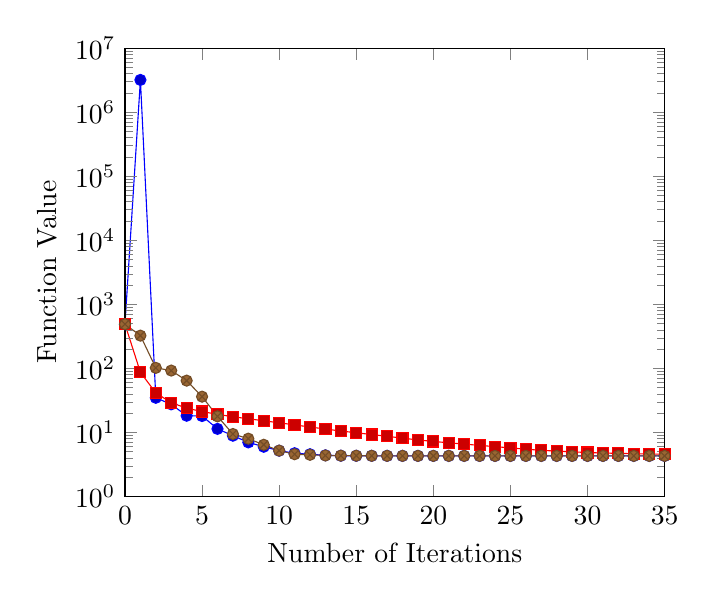
\begin{tikzpicture}

\begin{axis}[
xlabel={Number of Iterations},
ylabel={Function Value},
xmin=0, xmax=35,
ymin=1, ymax=10000000,
ymode=log,
axis on top
]
\addplot
coordinates {
(0,489.881511938848)
(1,3192254.85772505)
(2,34.7454630627093)
(3,27.4700063054781)
(4,18.2252052562127)
(5,18.0339938128533)
(6,11.3637878904689)
(7,8.895616996928)
(8,6.99254719962848)
(9,5.97893877098281)
(10,5.19063930967619)
(11,4.73456629491559)
(12,4.56721573152162)
(13,4.39185446923726)
(14,4.32837912703371)
(15,4.31896680094834)
(16,4.3109730327441)
(17,4.30900595602264)
(18,4.30563630693327)
(19,4.30322803013558)
(20,4.30150390633893)
(21,4.30080274657559)
(22,4.30030240409882)
(23,4.30019010402579)
(24,4.30012203632184)
(25,4.30009777305644)
(26,4.30006463492809)
(27,4.30004754413418)
(28,4.3000245981469)
(29,4.30001174039534)
(30,4.29999966823691)
(31,4.29999368795428)
(32,4.29998903159983)
(33,4.29998671986253)
(34,4.29998465332503)
(35,4.29998350130468)
(36,4.29998235635478)
(37,4.29998171580934)
(38,4.2999811507737)
(39,4.29998083490282)
(40,4.29998048802961)
(41,4.29998025566952)
(42,4.29998001759211)
(43,4.29997988412467)
(44,4.2999797816982)
(45,4.29997973234544)
(46,4.2999796933844)
(47,4.2999796729362)
(48,4.29997965211428)
(49,4.29997963847713)
(50,4.2999796218731)
(51,4.2999796105372)
(52,4.29997960077222)
(53,4.29997959599013)
(54,4.29997959260699)
(55,4.29997959096892)
(56,4.29997958961387)
(57,4.29997958887908)
(58,4.29997958810234)
(59,4.29997958758106)
(60,4.29997958692129)
(61,4.29997958646001)
(62,4.29997958606359)
(63,4.29997958586974)
(64,4.29997958572777)
(65,4.29997958565734)
(66,4.29997958559682)
(67,4.29997958556374)
(68,4.29997958552866)
(69,4.29997958550579)
(70,4.29997958547711)
(71,4.29997958545704)
(72,4.29997958543835)
(73,4.29997958542868)
(74,4.29997958542135)
(75,4.29997958541768)
(76,4.2999795854146)
(77,4.29997958541295)
(78,4.29997958541129)
(79,4.29997958541025)
(80,4.29997958540899)
(81,4.2999795854081)
(82,4.29997958540719)
(83,4.2999795854067)
(84,4.29997958540633)
(85,4.29997958540616)
(86,4.299979585406)
(87,4.29997958540592)
(88,4.29997958540585)
(89,4.2999795854058)
(90,4.29997958540575)
(91,4.29997958540571)
(92,4.29997958540567)
(93,4.29997958540564)
(94,4.29997958540562)
(95,4.29997958540561)
(96,4.29997958540561)
(97,4.29997958540561)
(98,4.2999795854056)
(99,4.2999795854056)
(100,4.2999795854056)
(101,4.2999795854056)
(102,4.29997958540559)
(103,4.29997958540559)
(104,4.29997958540559)

};
\addplot
coordinates {
(0,489.881511938848)
(1,86.8967090100459)
(2,41.3777498752359)
(3,29.1547588367561)
(4,23.908833449555)
(5,21.18010859399)
(6,19.1702332448616)
(7,17.5704039918483)
(8,16.3336871340434)
(9,15.2078805342798)
(10,14.1387183390872)
(11,13.107110529842)
(12,12.1555996095244)
(13,11.3023954775549)
(14,10.5259706926085)
(15,9.87789819688148)
(16,9.27278185151012)
(17,8.69908642190628)
(18,8.15179448966115)
(19,7.63210450062835)
(20,7.23896366022997)
(21,6.88719746681687)
(22,6.57391214381086)
(23,6.28071244385377)
(24,6.00040927525029)
(25,5.73286178243531)
(26,5.47745782324497)
(27,5.25622111192663)
(28,5.10749544967349)
(29,4.9786490193843)
(30,4.85751842347406)
(31,4.77081174582444)
(32,4.71009114241706)
(33,4.65679924321569)
(34,4.60850415850543)
(35,4.56393298979364)
(36,4.52229029845807)
(37,4.48302191327181)
(38,4.44861912456586)
(39,4.42283729991591)
(40,4.40166258304648)
(41,4.38341341211986)
(42,4.36747841558805)
(43,4.35475214890188)
(44,4.34822296180141)
(45,4.3432487364952)
(46,4.33928040336727)
(47,4.33602386223825)
(48,4.33329757331819)
(49,4.33097798692986)
(50,4.32897578993823)
(51,4.32722410158918)
(52,4.32567180920726)
(53,4.32427937723272)
(54,4.32301599325602)
(55,4.32185751895566)
(56,4.32078496965023)
(57,4.31978336335219)
(58,4.31888253917192)
(59,4.31804375125119)
(60,4.31725378705799)
(61,4.31650508771199)
(62,4.31579219940019)
(63,4.31511101876233)
(64,4.31445836075345)
(65,4.31383169117005)
(66,4.31322895106181)
(67,4.31264843640606)
(68,4.31208871304332)
(69,4.31154855513651)
(70,4.31102689984945)
(71,4.31052281348673)
(72,4.31003546588672)
(73,4.3095641108481)
(74,4.30910807102274)
(75,4.30866672615153)
(76,4.30823950382623)
(77,4.30782587217751)
(78,4.30742533404336)
(79,4.30703742228405)
(80,4.30666169599106)
(81,4.30629773739783)
(82,4.30594514934433)
(83,4.30560355318165)
(84,4.30527258702749)
(85,4.30495190430317)
(86,4.30464117249755)
(87,4.30434007211438)
(88,4.30404829576899)
(89,4.30376554740682)
(90,4.30349154162177)
(91,4.30322600305696)
(92,4.30296866587364)
(93,4.30273000566135)
(94,4.30252127163304)
(95,4.30233244722529)
(96,4.30216037067671)
(97,4.30200272587944)
(98,4.30185774525118)
(99,4.30172403457672)
(100,4.30160046166051)
(101,4.30148608293588)
(102,4.30138009412127)
(103,4.30128179655385)
(104,4.30119057388988)
(105,4.3011058757199)
(106,4.3010272058308)
(107,4.30095411361458)
(108,4.30088618762758)
(109,4.30082305063549)
(110,4.30076435569919)
(111,4.30070978300153)
(112,4.30065903721216)
(113,4.30061184525152)
(114,4.30056795435854)
(115,4.30052713039515)
(116,4.30048915634046)
(117,4.30045383094022)
(118,4.30042096748673)
(119,4.30039039271003)
(120,4.30036194576591)
(121,4.30033547730915)
(122,4.30031084864248)
(123,4.30028793093383)
(124,4.30026660449484)
(125,4.30024675811545)
(126,4.30022828844931)
(127,4.30021109944574)
(128,4.30019510182449)
(129,4.30018021258966)
(130,4.30016635457969)
(131,4.30015345605061)
(132,4.30014145028991)
(133,4.30013027525861)
(134,4.30011987325951)
(135,4.30011019062954)
(136,4.30010117745429)
(137,4.30009278730327)
(138,4.30008497698419)
(139,4.30007770631486)
(140,4.30007093791148)
(141,4.30006463699204)
(142,4.30005877119374)
(143,4.30005331040343)
(144,4.30004822660005)
(145,4.30004349370833)
(146,4.30003908746275)
(147,4.30003498528117)
(148,4.30003116614739)
(149,4.300027610502)
(150,4.30002430014078)
(151,4.30002121812048)
(152,4.30001834867099)
(153,4.30001567711377)
(154,4.30001318978607)
(155,4.30001087397026)
(156,4.3000087178283)
(157,4.30000671034064)
(158,4.30000484124952)
(159,4.30000310100609)
(160,4.30000148072128)
(161,4.29999997212016)
(162,4.29999856749932)
(163,4.29999725968736)
(164,4.29999604200804)
(165,4.29999490824605)
(166,4.2999938526151)
(167,4.29999286972824)
(168,4.29999195457029)
(169,4.29999110247213)
(170,4.29999030908675)
(171,4.29998957036704)
(172,4.29998888254508)
(173,4.29998824211278)
(174,4.29998764580404)
(175,4.29998709057797)
(176,4.29998657360336)
(177,4.29998609224423)
(178,4.29998564404633)
(179,4.2999852267246)
(180,4.29998483815154)
(181,4.29998447634625)
(182,4.29998413946443)
(183,4.29998382578886)
(184,4.29998353372067)
(185,4.29998326177124)
(186,4.29998300855446)
(187,4.29998277277981)
(188,4.29998255324565)
(189,4.29998234883319)
(190,4.2999821585007)
(191,4.29998198127823)
(192,4.29998181626268)
(193,4.29998166261315)
(194,4.29998151954672)
(195,4.29998138633435)
(196,4.29998126229728)
(197,4.29998114680348)
(198,4.29998103926448)
(199,4.29998093913234)
(200,4.29998084589687)
(201,4.29998075908303)
(202,4.29998067824851)
(203,4.29998060298144)
(204,4.29998053289836)
(205,4.29998046764221)
(206,4.29998040688051)
(207,4.29998035030371)
(208,4.29998029762355)
(209,4.29998024857167)
(210,4.29998020289814)
(211,4.2999801603703)
(212,4.29998012077148)
(213,4.29998008389993)
(214,4.29998004956783)
(215,4.29998001760027)
(216,4.29997998783439)
(217,4.29997996011855)
(218,4.29997993431157)
(219,4.29997991028196)
(220,4.29997988790732)
(221,4.29997986707367)
(222,4.29997984767486)
(223,4.29997982961209)
(224,4.29997981279333)
(225,4.2999797971329)
(226,4.29997978255103)
(227,4.29997976897343)
(228,4.29997975633094)
(229,4.29997974455916)
(230,4.29997973359812)
(231,4.29997972339197)
(232,4.29997971388873)
(233,4.29997970504)
(234,4.29997969680068)
(235,4.29997968912882)
(236,4.29997968198532)
(237,4.29997967533381)
(238,4.29997966914039)
(239,4.29997966337351)
(240,4.29997965800381)
(241,4.29997965300393)
(242,4.29997964834838)
(243,4.29997964401347)
(244,4.29997963997711)
(245,4.29997963621874)
(246,4.2999796327192)
(247,4.29997962946069)
(248,4.29997962642659)
(249,4.29997962360145)
(250,4.29997962097088)
(251,4.29997961852147)
(252,4.29997961624077)
(253,4.29997961411713)
(254,4.29997961213975)
(255,4.29997961029856)
(256,4.29997960858416)
(257,4.29997960698784)
(258,4.29997960550146)
(259,4.29997960411745)
(260,4.29997960282875)
(261,4.29997960162881)
(262,4.29997960051151)
(263,4.29997959947116)
(264,4.29997959850245)
(265,4.29997959760047)
(266,4.2999795967606)
(267,4.29997959597858)
(268,4.29997959525041)
(269,4.29997959457239)
(270,4.29997959394107)
(271,4.29997959335323)
(272,4.29997959280587)
(273,4.29997959229621)
(274,4.29997959182165)
(275,4.29997959137977)
(276,4.29997959096833)
(277,4.29997959058522)
(278,4.29997959022849)
(279,4.29997958989634)
(280,4.29997958958706)
(281,4.29997958929908)
(282,4.29997958903093)
(283,4.29997958878126)
(284,4.29997958854877)
(285,4.2999795883323)
(286,4.29997958813073)
(287,4.29997958794305)
(288,4.2999795877683)
(289,4.29997958760558)
(290,4.29997958745406)
(291,4.29997958731298)
(292,4.29997958718162)
(293,4.2999795870593)
(294,4.29997958694541)
(295,4.29997958683937)
(296,4.29997958674061)
(297,4.29997958664867)
(298,4.29997958656307)
(299,4.29997958648335)
(300,4.29997958640912)
(301,4.29997958634)
(302,4.29997958627565)
(303,4.29997958621573)
(304,4.29997958615994)
(305,4.29997958610798)
(306,4.29997958605961)
(307,4.29997958601457)
(308,4.29997958597262)
(309,4.29997958593358)
(310,4.29997958589721)
(311,4.29997958586335)
(312,4.29997958583183)
(313,4.29997958580247)
(314,4.29997958577514)
(315,4.29997958574969)
(316,4.29997958572599)
(317,4.29997958570392)
(318,4.29997958568338)
(319,4.29997958566424)
(320,4.29997958564643)
(321,4.29997958562984)
(322,4.2999795856144)
(323,4.29997958560002)
(324,4.29997958558663)
(325,4.29997958557416)
(326,4.29997958556255)
(327,4.29997958555174)
(328,4.29997958554167)
(329,4.2999795855323)
(330,4.29997958552358)
(331,4.29997958551545)
(332,4.29997958550788)
(333,4.29997958550084)
(334,4.29997958549428)
(335,4.29997958548817)
(336,4.29997958548249)
(337,4.29997958547718)
(338,4.29997958547225)
(339,4.29997958546766)
(340,4.29997958546339)
(341,4.29997958545941)
(342,4.2999795854557)
(343,4.29997958545225)
(344,4.29997958544904)
(345,4.29997958544604)
(346,4.29997958544326)
(347,4.29997958544067)
(348,4.29997958543825)
(349,4.299979585436)
(350,4.2999795854339)
(351,4.29997958543196)
(352,4.29997958543014)
(353,4.29997958542845)
(354,4.29997958542687)
(355,4.2999795854254)
(356,4.29997958542404)
(357,4.29997958542278)
(358,4.29997958542159)
(359,4.29997958542048)
(360,4.29997958541946)
(361,4.29997958541851)
(362,4.29997958541761)
(363,4.29997958541679)
(364,4.29997958541602)
(365,4.2999795854153)
(366,4.29997958541463)
(367,4.299979585414)
(368,4.29997958541343)
(369,4.29997958541288)
(370,4.29997958541239)
(371,4.29997958541192)
(372,4.29997958541148)
(373,4.29997958541107)
(374,4.29997958541069)
(375,4.29997958541035)
(376,4.29997958541002)
(377,4.29997958540971)
(378,4.29997958540943)
(379,4.29997958540916)
(380,4.29997958540892)
(381,4.29997958540869)
(382,4.29997958540848)
(383,4.29997958540828)
(384,4.29997958540809)
(385,4.29997958540792)
(386,4.29997958540776)
(387,4.29997958540761)
(388,4.29997958540747)
(389,4.29997958540734)
(390,4.29997958540722)
(391,4.29997958540711)
(392,4.299979585407)
(393,4.29997958540691)
(394,4.29997958540682)
(395,4.29997958540673)
(396,4.29997958540665)
(397,4.29997958540658)
(398,4.29997958540651)
(399,4.29997958540645)
(400,4.29997958540638)
(401,4.29997958540633)
(402,4.29997958540628)
(403,4.29997958540623)
(404,4.29997958540619)
(405,4.29997958540615)
(406,4.29997958540611)
(407,4.29997958540607)
(408,4.29997958540604)
(409,4.29997958540601)
(410,4.29997958540598)
(411,4.29997958540595)
(412,4.29997958540593)
(413,4.29997958540591)
(414,4.29997958540588)
(415,4.29997958540586)
(416,4.29997958540585)
(417,4.29997958540583)
(418,4.29997958540581)
(419,4.29997958540579)
(420,4.29997958540578)
(421,4.29997958540577)
(422,4.29997958540576)
(423,4.29997958540574)
(424,4.29997958540573)
(425,4.29997958540572)
(426,4.29997958540571)
(427,4.29997958540571)
(428,4.2999795854057)
(429,4.29997958540569)
(430,4.29997958540568)
(431,4.29997958540568)

};
\addplot 
coordinates {
(0,489.881511938848)
(1,324.751480131803)
(2,101.860905910834)
(3,92.4556878309931)
(4,64.4023284446456)
(5,36.1921402444228)
(6,17.8269186101206)
(7,9.44965000457534)
(8,7.99389900510047)
(9,6.415381070885)
(10,5.20308164302437)
(11,4.56865024856122)
(12,4.47411441266748)
(13,4.36669108343436)
(14,4.33992336163519)
(15,4.32877468307854)
(16,4.31568885009937)
(17,4.3117754388706)
(18,4.30840878190367)
(19,4.30693345750425)
(20,4.30566150357805)
(21,4.30425220896585)
(22,4.30273193981737)
(23,4.30192975792471)
(24,4.30087709687644)
(25,4.30070263381478)
(26,4.30038264553897)
(27,4.30023379602691)
(28,4.30013107634883)
(29,4.30007688083237)
(30,4.30003380601281)
(31,4.30001378001856)
(32,4.30000250844945)
(33,4.29999232569545)
(34,4.29998376898117)
(35,4.2999803375925)
(36,4.29997981120868)
(37,4.29997971651838)
(38,4.29997964749112)
(39,4.29997960114533)
(40,4.29997958897244)
(41,4.29997958714791)

};
\path [draw=black, fill opacity=0] (axis cs:13,9999999.99999998)--(axis cs:13,9999999.99999998);

\path [draw=black, fill opacity=0] (axis cs:35,13)--(axis cs:35,13);

\path [draw=black, fill opacity=0] (axis cs:13,1)--(axis cs:13,1);

\path [draw=black, fill opacity=0] (axis cs:0,13)--(axis cs:0,13);

\end{axis}

\end{tikzpicture}    
    \end{figure}


      hallo
  \end{frame}

  \plain{Questions?}

  \begin{frame}[allowframebreaks]\frametitle{Main References}

    \bibliography{refs}
    \bibliographystyle{abbrv}

  \end{frame}

\end{document}
